\documentclass[a4paper,14pt]{extarticle}
\usepackage[utf8x]{inputenc}
\usepackage[T1,T2A]{fontenc}
\usepackage[russian]{babel}
\usepackage{hyperref}
\usepackage{indentfirst}
\usepackage{listings}
\usepackage{color}
\usepackage{here}
\usepackage{array}
\usepackage{multirow}
\usepackage{graphicx}
\usepackage{caption}
\usepackage{subcaption}
\usepackage{chngcntr}
\usepackage[fleqn]{amsmath}
\usepackage{amssymb}
\usepackage{pgfplots}
\usepackage{pgfplotstable}
\counterwithin{figure}{section}
\counterwithin{equation}{section}
\counterwithin{table}{section}
\usepackage{tabularx}

%% Поля подписи и даты
\newcommand{\sign}[1][5cm]{%
\makebox[#1]{\hrulefill}
}

\usepackage[left=2cm,right=2cm,
top=2cm,bottom=2cm,bindingoffset=0cm]{geometry}


\begin{document}	% начало документа

\begin{titlepage}	% начало титульной страницы

	\begin{center}		% выравнивание по центру

		\large Санкт-Петербургский Политехнический Университет Петра Великого\\
		\large Институт компьютерных наук и технологий \\
		\large Кафедра компьютерных систем и программных технологий\\[4cm]
		% название института, затем отступ 6см
		
		 \huge Вычислительная математика\\[0.3cm] % название работы, затем отступ 0,5см
		 \large Расчётное задание №2\\[0.1cm]
		 \large Интерполяция\\[8cm]

	\end{center}


	\begin{flushright} % выравнивание по правому краю
		\begin{minipage}{0.35\textwidth} % врезка в половину ширины текста
			\begin{flushleft} % выровнять её содержимое по левому краю

				\large\textbf{Работу выполнил:}\\
				\large Ламтев А.Ю.\\
				\large {Группа:} 23501/4\\
				
				\large \textbf{Преподаватель:}\\
				\large Цыган В.Н.

			\end{flushleft}
		\end{minipage}
	\end{flushright}
	
	\vfill % заполнить всё доступное ниже пространство

	\begin{center}
	\large Санкт-Петербург\\
	\large \the\year % вывести дату
	\end{center} % закончить выравнивание по центру

\thispagestyle{empty} % не нумеровать страницу
\end{titlepage} % конец титульной страницы

\vfill % заполнить всё доступное ниже пространство


\section{Задание}

Аппроксимировать функцию 

\begin{displaymath}
f(x) = \frac{4}{4 + 5 \cdot x}
\end{displaymath}

на промежутке $\Big [ 0, 1 \Big ]$ методом наименьших квадратов с использованием:

\begin{enumerate}

\item Полинома второй степени $Q_2(x) = a_0 + a_1x + a_2x^2$

\item Ортонормированных многочленов, которые предварительно необходимо построить методом Грама-Шмидта по системе функций: $\phi_0(x) = 1$, $\phi_1(x) = x$, $\phi_2(x) = x^2$

\item Ортогональных многочленов Лежандра порядка до двух включительно.

\item Ортогональных многочленов Чебышева порядка до двух включительно.

\end{enumerate}

Построить для интервала $\Big [ 0, 1 \Big ]$ график исходной функции, графики аппроксимирующих функций и графики погрешностей аппроксимации 

$\varepsilon = f(x) - Q(x)$.

\section{Решение}

\begin{displaymath}
Q_2(x) = a_0 \cdot \phi_0(x) + a_1 \cdot \phi_1(x) + a_2 \cdot \phi_2(x)
\end{displaymath}

\begin{displaymath}
\rho^2 = \int_a^b P(x (Q_2(x) - f(x))^2 dx = \int_a^b P(x) (a_0 \phi_0(x) + a_1 \phi_1(x) + a_2 \phi_2(x) - f(x))^2 dx \  \  \ (\bigstar)
\end{displaymath}

$\bigstar \rightarrow minimum :$\\[1mm]

$
 \begin{cases}
  \frac{\partial \rho^2}{\partial a_0} = 2 \int_a^b P(x) (a_0 \phi_0(x) + a_1 \phi_1(x) + a_2 \phi_2(x) - f(x)) \phi_0 dx = 0
   \\[2mm]
  \frac{\partial \rho^2}{\partial a_1} = 2 \int_a^b P(x) (a_0 \phi_0(x) + a_1 \phi_1(x) + a_2 \phi_2(x) - f(x)) \phi_1 dx = 0
   \\[2mm]
  \frac{\partial \rho^2}{\partial a_2} = 2 \int_a^b P(x) (a_0 \phi_0(x) + a_1 \phi_1(x) + a_2 \phi_2(x) - f(x)) \phi_2 dx = 0
 \end{cases}
$\\[1mm]

\begin{displaymath}
\Big (\phi_k, \phi_i \Big ) = \frac{1}{b - a} \cdot \int_a^b P(x) \cdot \phi_k(x) \cdot \phi_i(x)dx
\end{displaymath}

$
\begin{pmatrix}
(\phi_0, \phi_0) & (\phi_1, \phi_0) & (\phi_2, \phi_0)
\\
(\phi_0, \phi_1) & (\phi_1, \phi_1) & (\phi_2, \phi_1)
\\
(\phi_0, \phi_2) & (\phi_1, \phi_2) & (\phi_2, \phi_2)
\end{pmatrix}
\cdot
\begin{pmatrix}
a_0
\\
a_1
\\
a_2
\end{pmatrix}
=
\begin{pmatrix}
(f, \phi_0)
\\
(f, \phi_1)
\\
(f, \phi_2)
\end{pmatrix}
$


$a = 0, b = 1$

\subsection{С использованием полинома второй степени}

$\phi_0(x) \equiv 1, \phi_1(x) = x, \phi_2(x) = x^2, P(x) \equiv 1$

\begin{displaymath}
Q_2(x) = a_0 + a_1 \cdot x + a_2 \cdot x^2
\end{displaymath}
\begin{displaymath}
(\phi_0, \phi_0) = 1 \ \ (\phi_1, \phi_0) = (\phi_0, \phi_1) = \frac{1}{2}
\end{displaymath}
\begin{displaymath}
(\phi_1, \phi_1) = \frac{1}{3} \ \ (\phi_2, \phi_0) = (\phi_0, \phi_2) = \frac{1}{3}
\end{displaymath}
\begin{displaymath}
(\phi_2, \phi_2) = \frac{1}{5} \ \ (\phi_2, \phi_1) = (\phi_1, \phi_2) = \frac{1}{4}
\end{displaymath}

\begin{displaymath}
(f, \phi_0) = \int_0^1 \frac{4}{4 + 5 \cdot x} \cdot 1 dx = 0.6487441729730634
\end{displaymath}
\begin{displaymath}
(f, \phi_1) = \int_0^1 \frac{4}{4 + 5 \cdot x} \cdot x dx = 0.2810046616215496
\end{displaymath}
\begin{displaymath}
(f, \phi_2) = \int_0^1 \frac{4}{4 + 5 \cdot x} \cdot x^2 dx = 0.1751962707027603
\end{displaymath}

$
\begin{pmatrix}
1 & \frac{1}{2} & \frac{1}{3}
\\
\frac{1}{2} & \frac{1}{3} & \frac{1}{4}
\\
\frac{1}{3} & \frac{1}{4} & \frac{1}{5}
\end{pmatrix}
\cdot
\begin{pmatrix}
a_0
\\
a_1
\\
a_2
\end{pmatrix}
=
\begin{pmatrix}
0.6487441729730634
\\
0.2810046616215496
\\
0.1751962707027603
\end{pmatrix}
$\\[1mm]

$
 \begin{cases}
  a_0 = 0.9784178594645938
\\
  a_1 = -0.9372239221896193
\\
  a_2 = 0.416814823809832
 \end{cases}
$\\[1mm]

\begin{displaymath}
Q_2(x) = 0.416814823809832 \cdot x^2 - 0.9372239221896193 \cdot x + 0.9784178594645938
\end{displaymath}

\begin{figure}[H]
	\begin{center}
		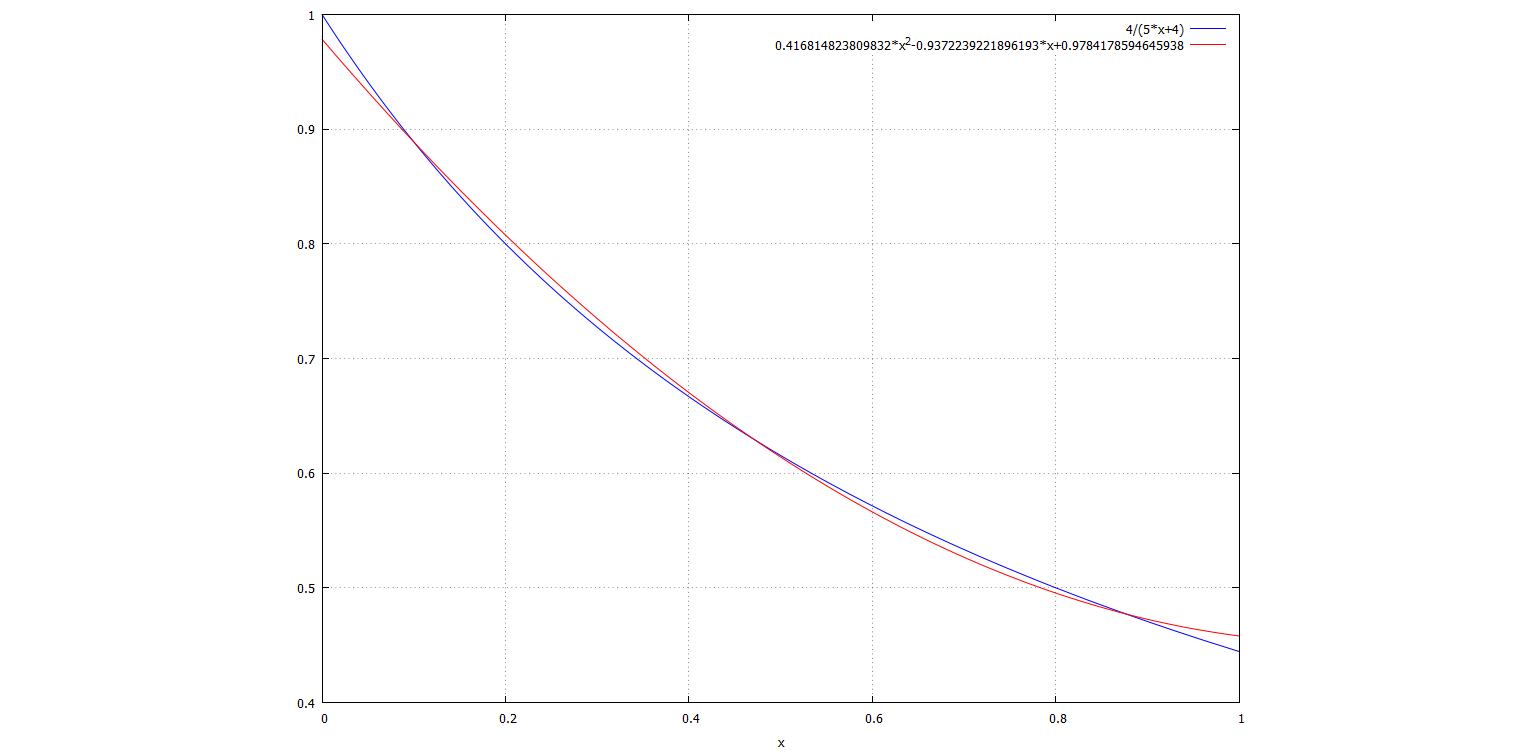
\includegraphics[width=19cm]{polynoms.png}
		\caption{График исходной функции и аппроксимирующей функции} 
		\label{pic:2:1:1}
	\end{center}
\end{figure}

\begin{figure}[H]
	\begin{center}
		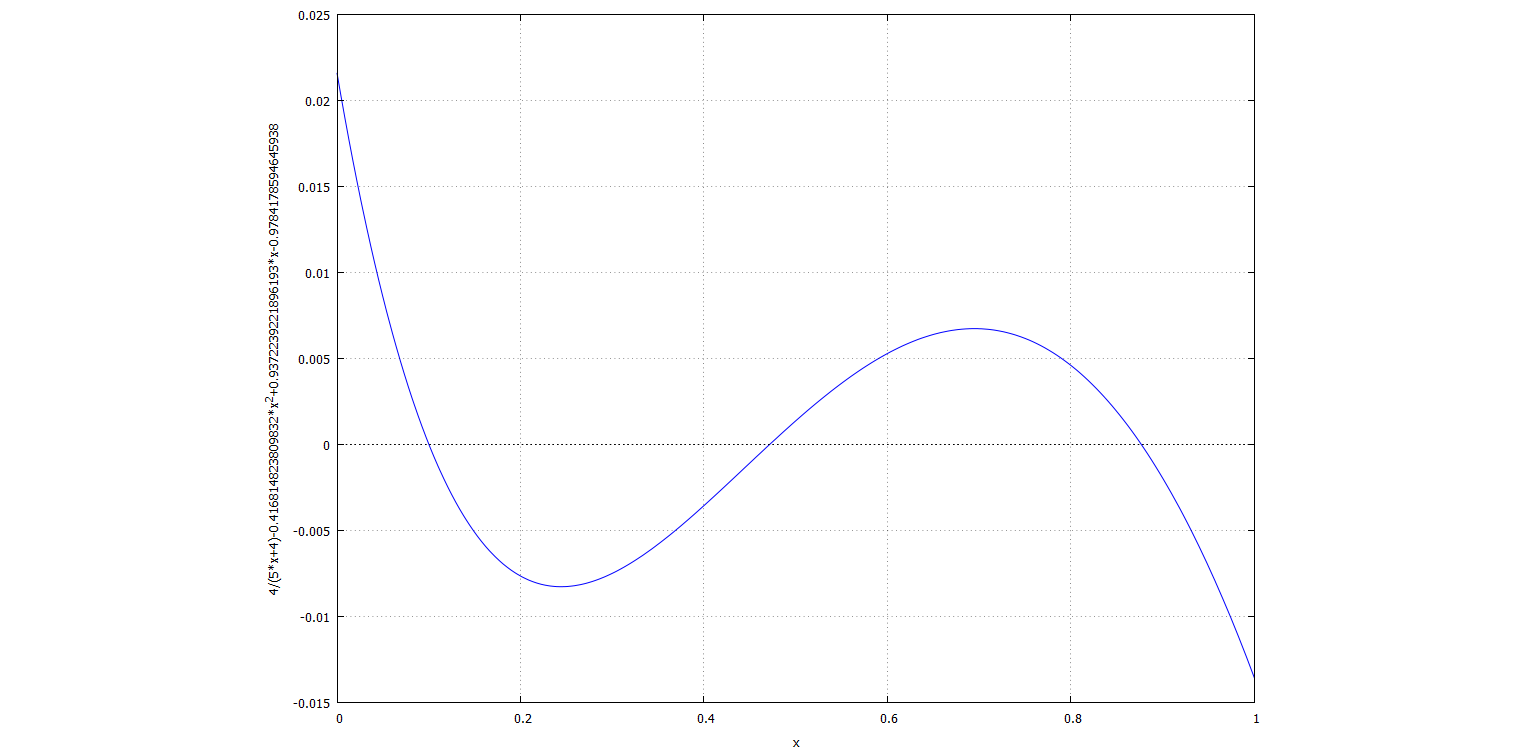
\includegraphics[width=19cm]{e_polynoms.png}
		\caption{График погрешности аппроксимирующей функции} 
		\label{pic:2:1:2}
	\end{center}
\end{figure}

\newpage

\subsection{С помощью ортонормированных многочленов}

$f_0(x) \equiv 1, f_1(x) = x, f_2(x) = x^2, P(x) \equiv 1$

\begin{displaymath}
g_0(x) = f_0(x) = 1
\end{displaymath}
\begin{displaymath}
g_1(x) = f_1(x) - \frac{\int_0^1 f_1(x) g_0(x)dx}{\int_0^1 (g_0(x))^2dx}g_0(x) = x - \frac{1}{2}
\end{displaymath}
\begin{displaymath}
g_2(x) = f_2(x) - \frac{\int_0^1 f_2(x) g_0(x)dx}{\int_0^1 (g_0(x))^2dx}g_0(x) - \frac{\int_0^1 f_2(x) g_1(x)dx}{\int_0^1 (g_1(x))^2dx}g_1(x) = x^2 - x + \frac{1}{6}
\end{displaymath}

\begin{displaymath}
\tilde{g}(x) = \frac{g(x)}{\alpha} \Rightarrow \int_0^1 \frac{(g(x))^2dx}{\alpha^2} = 1 \Rightarrow \alpha = \sqrt{\int_0^1 (g(x))^2dx}
\end{displaymath}

\begin{displaymath}
\alpha_0 = 1, \tilde{g}_0(x) = 1
\end{displaymath}
\begin{displaymath}
\alpha_1 = \frac{1}{2 \sqrt{3}}, \tilde{g}_1(x) = \sqrt{3} \cdot (2x - 1)
\end{displaymath}
\begin{displaymath}
\alpha_2 = \frac{1}{2 \sqrt{3}}, \tilde{g}_2(x) = \sqrt{5} \cdot (6x^2 - 6x + 1)
\end{displaymath}

\begin{displaymath}
Q_2(x) = a_0 + a_1 \sqrt{3}(2x - 1) + a_2 \sqrt{5}(6x^2 - 6x + 1)
\end{displaymath}

\begin{displaymath}
(\phi_0, \phi_0) = 1 \ \ (\phi_1, \phi_0) = (\phi_0, \phi_1) = 0
\end{displaymath}
\begin{displaymath}
(\phi_1, \phi_1) = 1 \ \ (\phi_2, \phi_0) = (\phi_0, \phi_2) = 0
\end{displaymath}
\begin{displaymath}
(\phi_2, \phi_2) = 1 \ \ (\phi_2, \phi_1) = (\phi_1, \phi_2) = 0
\end{displaymath}

\begin{displaymath}
(f, \phi_0) = \int_0^1 \frac{4}{4 + 5 \cdot x} \cdot 1 dx = 0.6487441729730634
\end{displaymath}
\begin{displaymath}
(f, \phi_1) = \int_0^1 \frac{4}{4 + 5 \cdot x} \cdot \sqrt{3} (2x - 1) dx = -0.1502291665191494
\end{displaymath}
\begin{displaymath}
(f, \phi_2) = \int_0^1 \frac{4}{4 + 5 \cdot x} \cdot \sqrt{5} (6x^2 - 6x + 1) dx = 0.03106754266894511
\end{displaymath}

$
\begin{pmatrix}
1 & 0 & 0
\\
0 & 1 & 0
\\
0 & 0 & 1
\end{pmatrix}
\cdot
\begin{pmatrix}
a_0
\\
a_1
\\
a_2
\end{pmatrix}
=
\begin{pmatrix}
0.6487441729730634
\\
-0.1502291665191494
\\
0.03106754266894511
\end{pmatrix}
$\\[1mm]

$
 \begin{cases}
  a_0 = 0.6487441729730634
\\
  a_1 = -0.1502291665191494
\\
  a_2 = 0.03106754266894511
 \end{cases}
$\\[1mm]

\begin{displaymath}
Q_2(x) = 0.4168148238098192 \cdot x^2 - 0.9372239221896032 \cdot x + 0.9784178594645919
\end{displaymath}

\begin{figure}[H]
	\begin{center}
		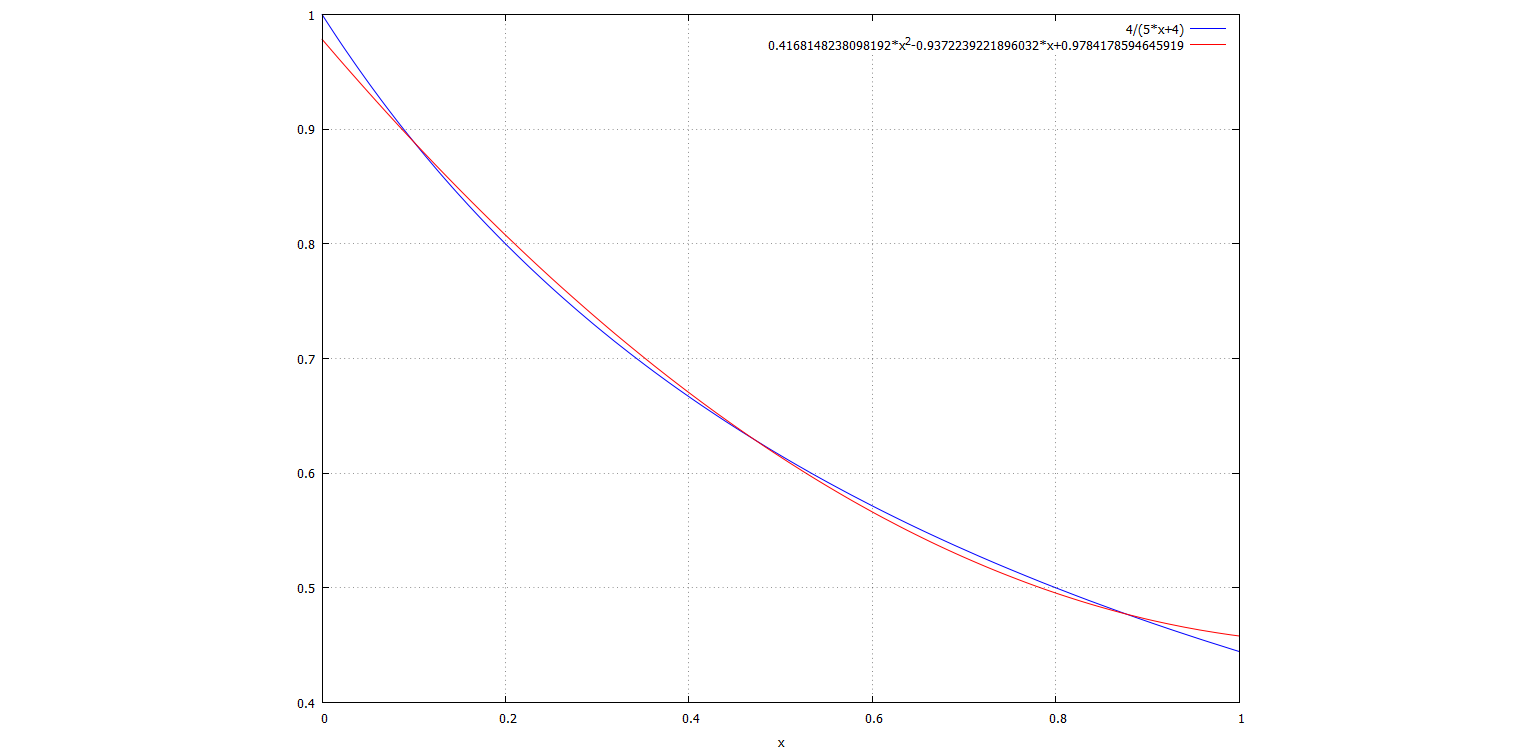
\includegraphics[width=19cm]{ortonorm.png}
		\caption{График исходной функции и аппроксимирующей функции} 
		\label{pic:2:2:1}
	\end{center}
\end{figure}

\begin{figure}[H]
	\begin{center}
		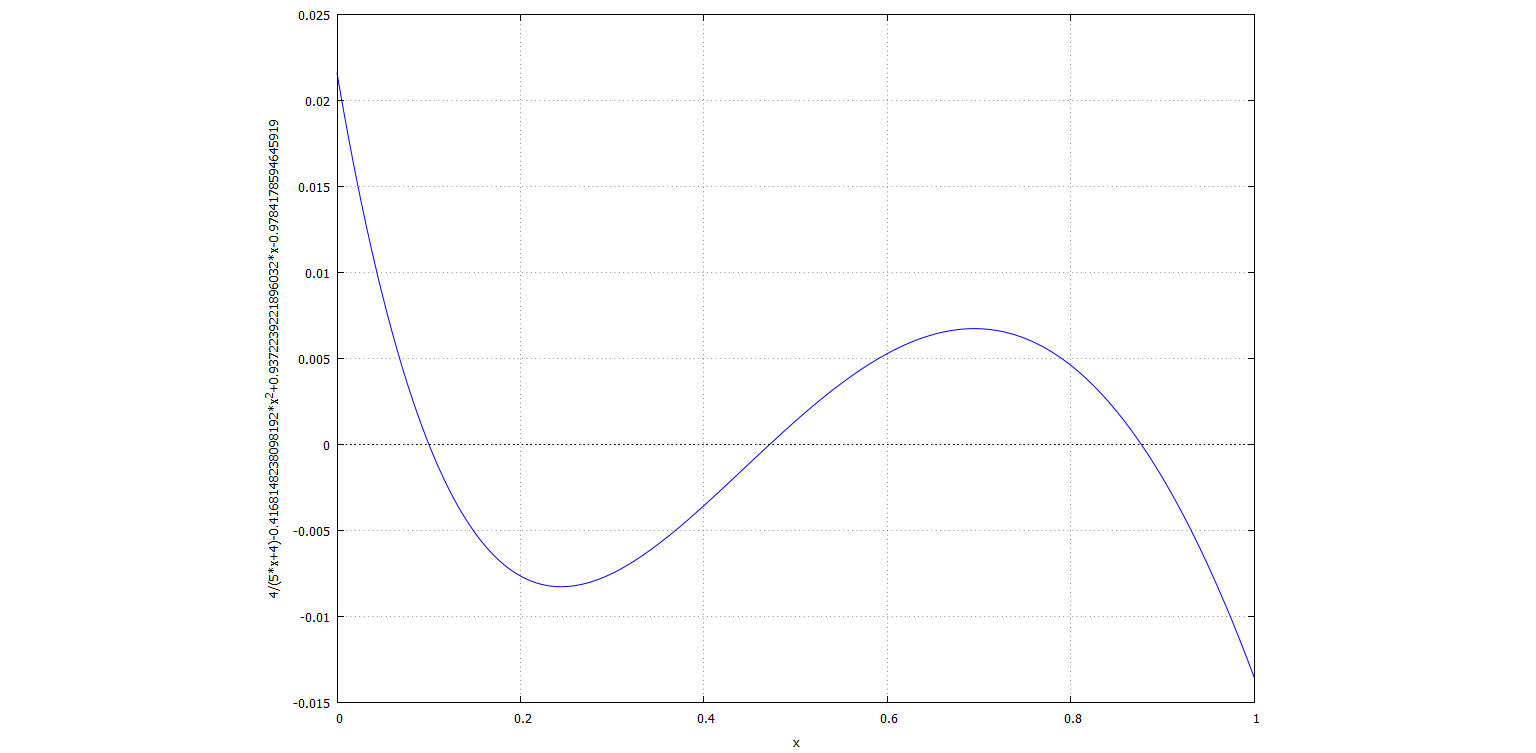
\includegraphics[width=19cm]{e_ortonorm.png}
		\caption{График погрешности аппроксимирующей функции} 
		\label{pic:2:2:2}
	\end{center}
\end{figure}

\subsection{С помощью ортогональных многочленов Лежандра порядка до двух включительно}

$P(x) \equiv 1$

\begin{displaymath}
L_0(t) = 1
\end{displaymath}
\begin{displaymath}
L_1(t) = t
\end{displaymath}
\begin{displaymath}
L_2(t) = \frac{1}{2} \cdot (3t^2 - 1)
\end{displaymath}

\begin{displaymath}
\int_{-1}^{1} L_i(t) L_k(t) dt = \begin{cases} 0, k \neq i \\ \frac{2}{2k + 1}, k = i \end{cases}
\end{displaymath}

\begin{displaymath}
x = \frac{a + b}{2} + \frac{b - a}{2} t \Rightarrow t = \frac{2x - a - b}{b - a} = 2x - 1
\end{displaymath}

\begin{displaymath}
L_0(x) = 1
\end{displaymath}
\begin{displaymath}
L_1(x) = 2x - 1
\end{displaymath}
\begin{displaymath}
L_2(x) = 6x^2 - 6x + 1
\end{displaymath}

\begin{displaymath}
\int_0^1 L_i(2x - 1) L_k(2x - 1) dx = \begin{cases} 0, k \neq i \\ \frac{2}{2k + 1} \cdot \frac{1}{2}, k = i \end{cases}
\end{displaymath}

\begin{displaymath}
Q_2(x) = a_0 + a_1 \cdot (2x - 1) + a_2 \cdot (6x^2 - 6x + 1)
\end{displaymath}

\begin{displaymath}
(\phi_0, \phi_0) = 1 \ \ (\phi_1, \phi_0) = (\phi_0, \phi_1) = 0
\end{displaymath}
\begin{displaymath}
(\phi_1, \phi_1) = \frac{1}{3} \ \ (\phi_2, \phi_0) = (\phi_0, \phi_2) = 0
\end{displaymath}
\begin{displaymath}
(\phi_2, \phi_2) = \frac{1}{5} \ \ (\phi_2, \phi_1) = (\phi_1, \phi_2) = 0
\end{displaymath}

\begin{displaymath}
(f, \phi_0) = \int_0^1 \frac{4}{4 + 5 \cdot x} \cdot 1 dx = 0.6487441729730634
\end{displaymath}
\begin{displaymath}
(f, \phi_1) = \int_0^1 \frac{4}{4 + 5 \cdot x} \cdot (2x - 1) dx = -0.08673484972996404
\end{displaymath}
\begin{displaymath}
(f, \phi_2) = \int_0^1 \frac{4}{4 + 5 \cdot x} \cdot (6x^2 - 6x + 1) dx = 0.0138938274603273
\end{displaymath}

$
\begin{pmatrix}
1 & 0 & 0
\\
0 & \frac{1}{3} & 0
\\
0 & 0 & \frac{1}{5}
\end{pmatrix}
\cdot
\begin{pmatrix}
a_0
\\
a_1
\\
a_2
\end{pmatrix}
=
\begin{pmatrix}
0.6487441729730634
\\
-0.08673484972996404
\\
0.0138938274603273
\end{pmatrix}
$\\[1mm]

$
 \begin{cases}
  a_0 = 0.6487441729730634
\\
  a_1 = -0.2602045491898922
\\
  a_2 = 0.06946913730163651
 \end{cases}
$\\[1mm]

\begin{displaymath}
Q_2(x) = 0.416814823809819 \cdot x^2 - 0.9372239221896035 \cdot x + 0.9784178594645921
\end{displaymath}

\begin{figure}[H]
	\begin{center}
		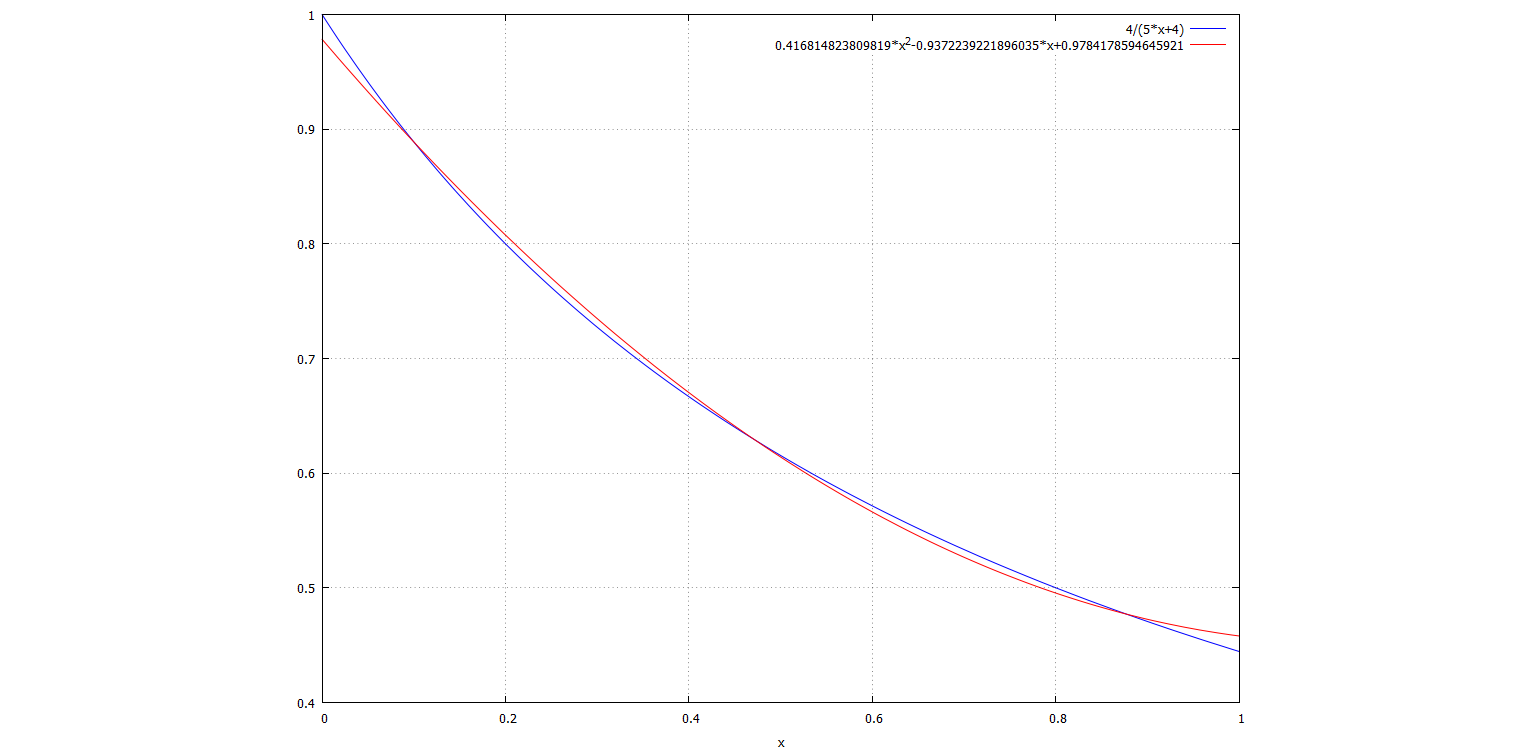
\includegraphics[width=19cm]{legandre.png}
		\caption{График исходной функции и аппроксимирующей функции} 
		\label{pic:2:3:1}
	\end{center}
\end{figure}

\begin{figure}[H]
	\begin{center}
		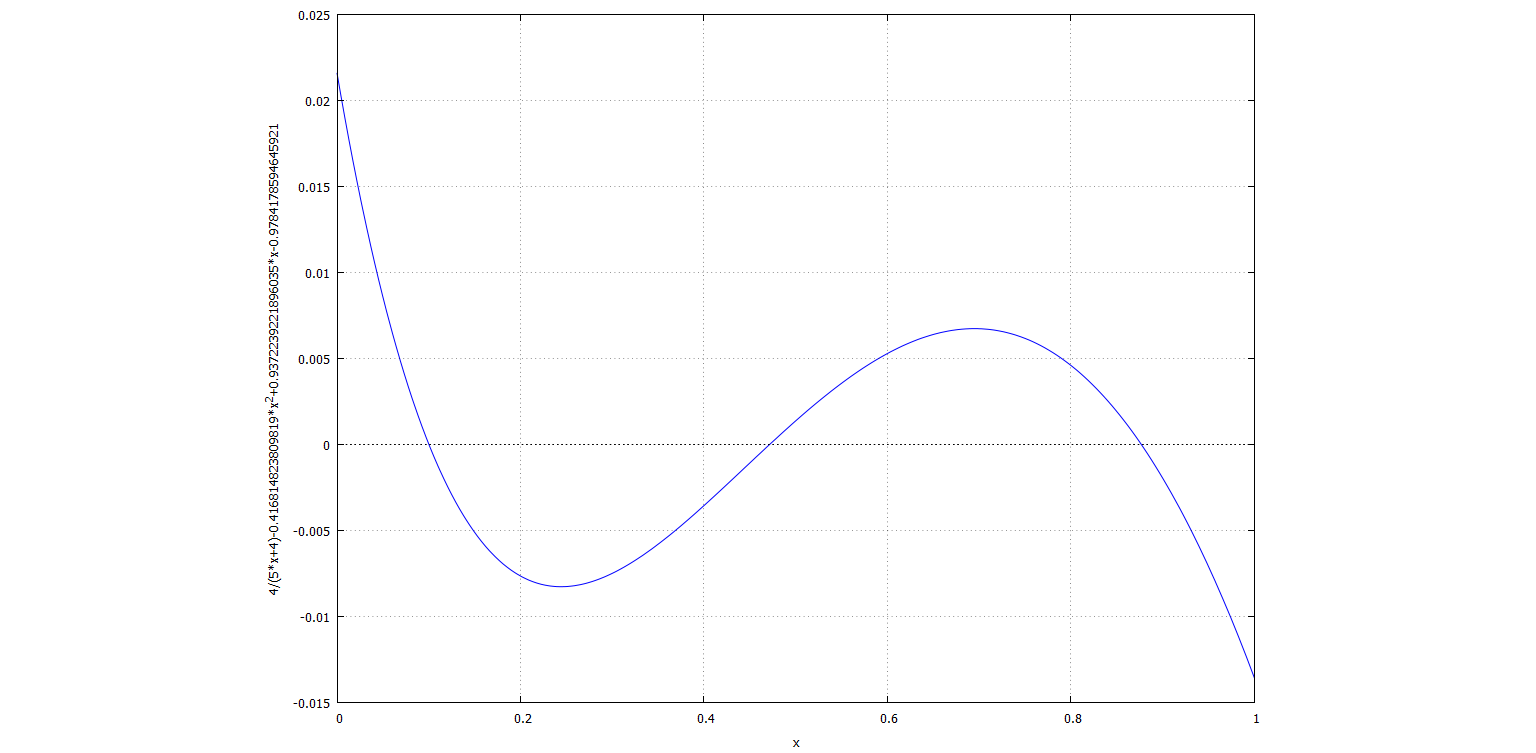
\includegraphics[width=19cm]{e_legandre.png}
		\caption{График погрешности аппроксимирующей функции} 
		\label{pic:2:3:2}
	\end{center}
\end{figure}

\newpage

\subsection{С помощью ортогональных многочленов Чебышева порядка до двух включительно}

$P(x) = \frac{1}{\sqrt{1 - t^2}}$

\begin{displaymath}
T_0(t) = 1
\end{displaymath}
\begin{displaymath}
T_1(t) = t
\end{displaymath}
\begin{displaymath}
T_2(t) = 2t^2 - 1
\end{displaymath}

\begin{displaymath}
\int_{-1}^{1} T_i(t) T_k(t) \frac{1}{\sqrt{1 - t^2}} dt = \begin{cases} 0, k \neq i \\ \frac{\pi}{2}, k = i \neq 0 \\ \pi, k = i = 0 \end{cases}
\end{displaymath}

\begin{displaymath}
x = \frac{a + b}{2} + \frac{b - a}{2} t \Rightarrow t = \frac{2x - a - b}{b - a} = 2x - 1
\end{displaymath}

\begin{displaymath}
T_0(x) = 1
\end{displaymath}
\begin{displaymath}
T_1(x) = 2x - 1
\end{displaymath}
\begin{displaymath}
T_2(x) = 8x^2 - 8x + 1
\end{displaymath}
\begin{displaymath}
\int_0^1 T_i(2x - 1) T_k(2x - 1)\frac{1}{2 \sqrt{x - x^2}} dx = \begin{cases} 0, k \neq i \\ \frac{\pi}{2} \cdot \frac{1}{2}, k = i \neq 0 \\ \pi \cdot \frac{1}{2}, k = i = 0 \end{cases}
\end{displaymath}

\begin{displaymath}
Q_2(x) = a_0 + a_1 \cdot (2x - 1) + a_2 \cdot (8x^2 - 8x + 1)
\end{displaymath}

\begin{displaymath}
(\phi_0, \phi_0) = \frac{\pi}{2} \ \ (\phi_1, \phi_0) = (\phi_0, \phi_1) = 0
\end{displaymath}
\begin{displaymath}
(\phi_1, \phi_1) = \frac{\pi}{4} \ \ (\phi_2, \phi_0) = (\phi_0, \phi_2) = 0
\end{displaymath}
\begin{displaymath}
(\phi_2, \phi_2) = \frac{\pi}{4} \ \ (\phi_2, \phi_1) = (\phi_1, \phi_2) = 0
\end{displaymath}

\begin{displaymath}
(f, \phi_0) = \int_0^1 \frac{4}{4 + 5 \cdot x} \cdot \frac{1}{2 \sqrt{x - x^2}} dx = 1.047197551196598
\end{displaymath}
\begin{displaymath}
(f, \phi_1) = \int_0^1 \frac{4}{4 + 5 \cdot x} \cdot (2x - 1) \frac{1}{2 \sqrt{x - x^2}} dx = -0.2094395102393195
\end{displaymath}
\begin{displaymath}
(f, \phi_2) = \int_0^1 \frac{4}{4 + 5 \cdot x} \cdot (8x^2 - 8x + 1) \frac{1}{2 \sqrt{x - x^2}} dx = 0.04188790204786391
\end{displaymath}

$
\begin{pmatrix}
\frac{\pi}{2} & 0 & 0
\\
0 & \frac{\pi}{4} & 0
\\
0 & 0 & \frac{\pi}{4}
\end{pmatrix}
\cdot
\begin{pmatrix}
a_0
\\
a_1
\\
a_2
\end{pmatrix}
=
\begin{pmatrix}
1.047197551196598
\\
-0.2094395102393195
\\
0.04188790204786391
\end{pmatrix}
$\\[1mm]

$
 \begin{cases}
  a_0 = 0.6666666666666671
\\
  a_1 = -0.2666666666666667
\\
  a_2 = 0.05333333333333334
 \end{cases}
$\\[1mm]

\begin{displaymath}
Q_2(x) = 0.4266666666666667 \cdot x^2 - 0.9600000000000002 \cdot x + 0.9866666666666671
\end{displaymath}

\begin{figure}[H]
	\begin{center}
		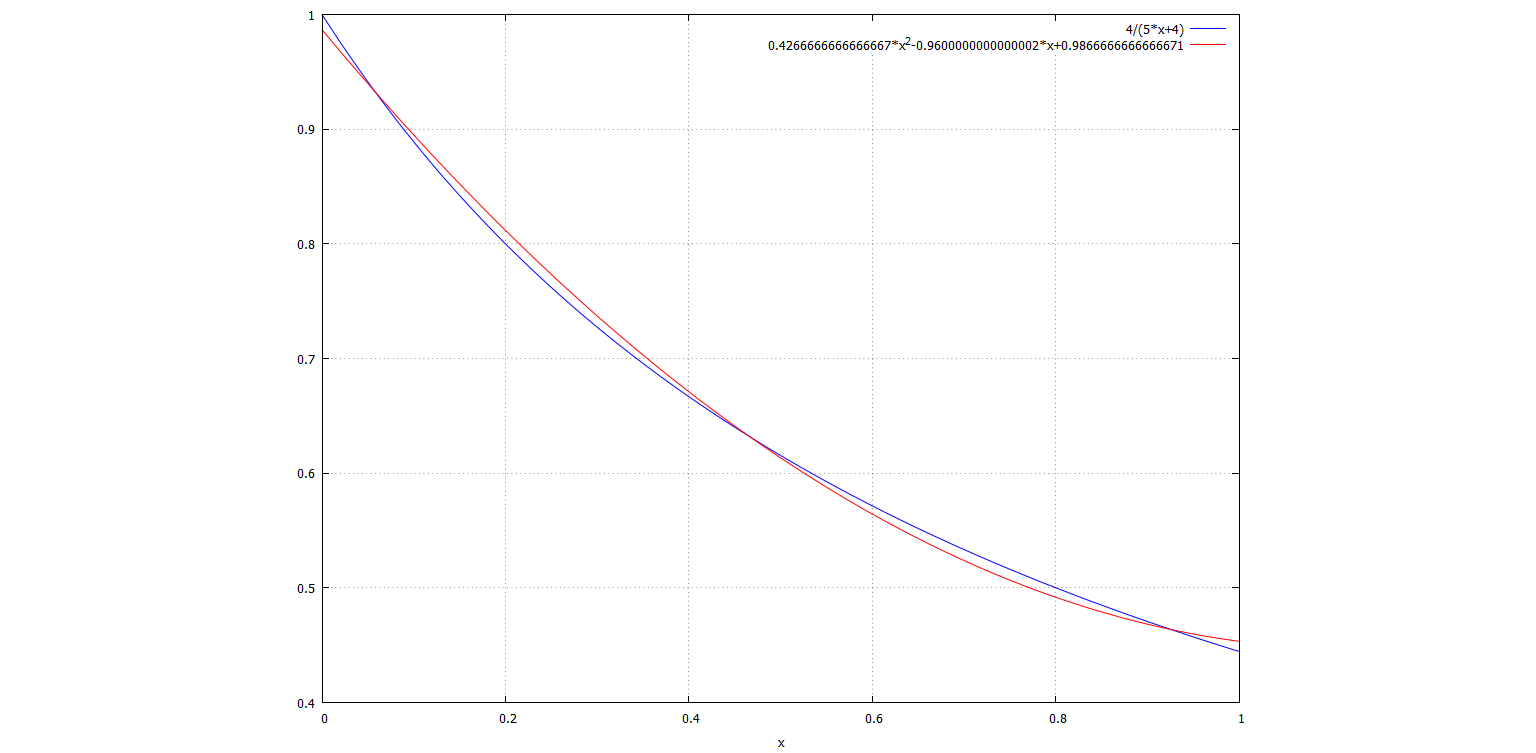
\includegraphics[width=19cm]{chebyshev.png}
		\caption{График исходной функции и аппроксимирующей функции} 
		\label{pic:2:4:1}
	\end{center}
\end{figure}

\begin{figure}[H]
	\begin{center}
		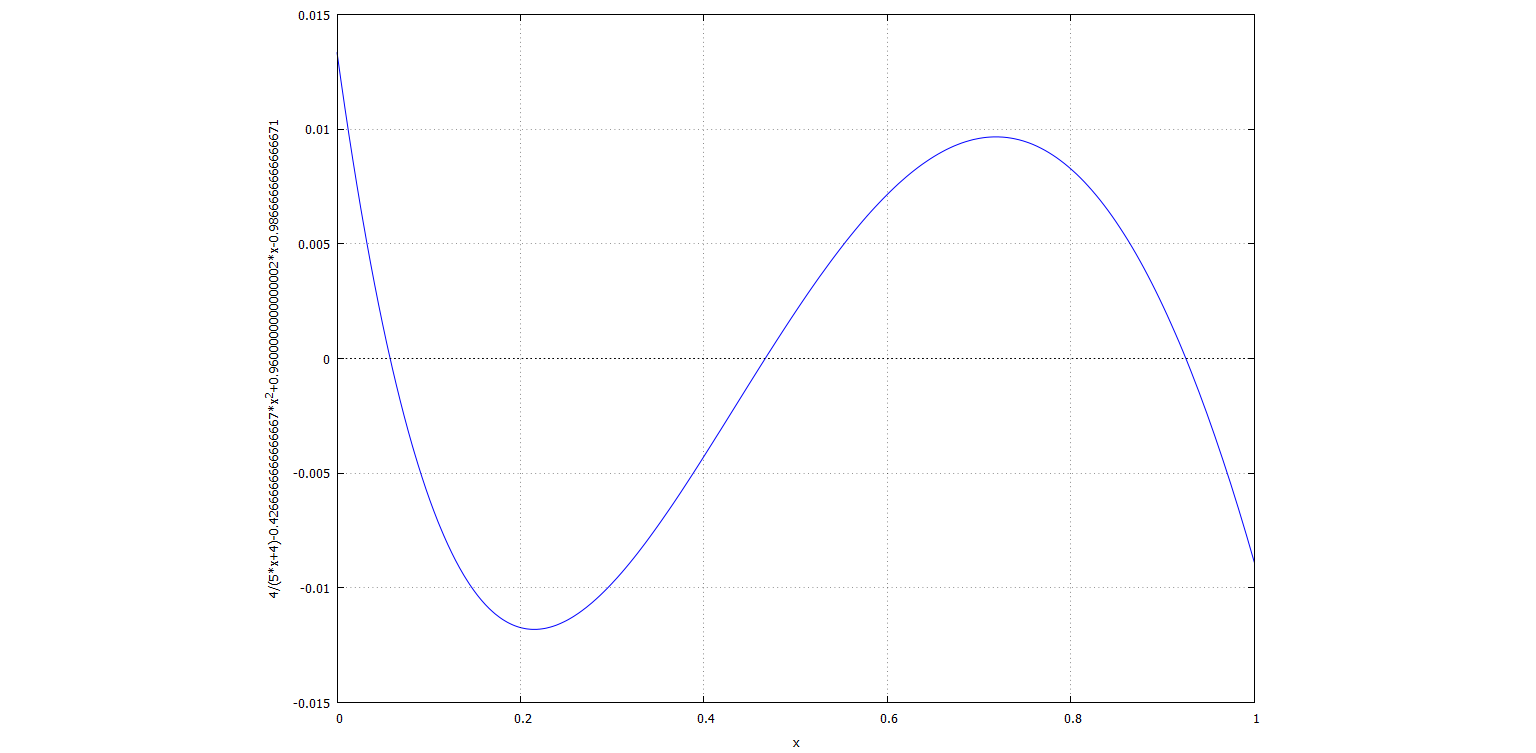
\includegraphics[width=19cm]{e_chebyshev.png}
		\caption{График погрешности аппроксимирующей функции} 
		\label{pic:2:4:2}
	\end{center}
\end{figure}

\end{document}
